\documentclass[conference]{IEEEtran}
\IEEEoverridecommandlockouts
% IEEE conference template (paper/confrence template, 10-17-19), compiled with XeLaTeX (tectonic) for the
% Persian examples. fontspec and the Persian font MUST be loaded before newtxtext.
\usepackage{fontspec}
\newfontfamily\persianfont[Script=Arabic]{Noto Naskh Arabic}
\TeXXeTstate=1
\newcommand{\fa}[1]{{\persianfont\beginR #1\endR}}
\usepackage{cite}
\usepackage{amsmath,amssymb}
\usepackage{newtxtext}
\usepackage{newtxmath}
\usepackage{graphicx}
\usepackage{textcomp}
\usepackage{xcolor}
\usepackage{booktabs}
\usepackage{tikz}
\usetikzlibrary{arrows.meta}
\usepackage[hidelinks]{hyperref}
% Every reported number traces to persian_tts/research/PROGRESS.md. To mark them for checking,
% use \newcommand{\RES}[1]{\textcolor{red}{#1}}.
\newcommand{\RES}[1]{#1}
\newcommand{\CODEURL}{\url{https://github.com/abolfazltorbat/persian_tts}}

\begin{document}

\title{Speaking Through the Prompt: Training-Free Robustness and Expressive Prosody for a Small CPU
Persian Text-to-Speech Model}

\author{\IEEEauthorblockN{Abolfazl Nejatian\textsuperscript{1,$\ast$}, Mehdi Alimohammadi\textsuperscript{2}, and
Amirhossein Parsa\textsuperscript{3}}
\IEEEauthorblockA{\textsuperscript{1}\textit{Faculty of Computer Engineering, Shahrood University of Technology},
Shahrood, Iran\\
\textsuperscript{2}\textit{Department of Electrical Engineering, Center of Excellence on Soft Computing and
Intelligent Information Processing,}\\ \textit{Ferdowsi University of Mashhad}, Mashhad, Iran\\
\textsuperscript{3}\textit{Faculty of Electrical Engineering, Shahid Beheshti University}, Tehran, Iran\\
EMAIL-1, EMAIL-2, EMAIL-3}}

\maketitle

\begin{abstract}
Small continuation text-to-speech (TTS) models now run in real time on a laptop CPU, but in practice they
fail in two ways that their size and training rule out fixing by retraining: they garble short utterances,
and, trained on text stripped of punctuation, they read every question and exclamation as a flat statement.
We study both in a public 110M-parameter Persian model and show that the model's second input --- the voice
prompt it continues --- is a control surface that solves both at inference time. \emph{Robustness:} failures
depend on how the prompt \emph{ends}. The model was trained to continue the prompt's own utterance, but at
inference its text is a new sentence; extending the reference clip with the model's own reading of one
neutral sentence makes every prompt end at a finished sentence, so the text reads as the next sentence,
which halves failed renders on held-out short sentences (\RES{24$\to$12} of \RES{900}; on nine further speakers
\RES{69$\to$28}) and rescues a clip cut mid-clause (\RES{44\%$\to$3\%} error) at no per-request cost. \emph{Expressiveness:} the prompt also carries register
and pitch range; a re-pitched, widened copy of that reading makes the model itself speak exclamations and
surprise livelier (pitch range \RES{+38\%}), while a light rule restores only what no prompt can --- the
sentence ending --- and a loudness plan spans the text. Yes/no questions are then heard as questions three
times as often by a recogniser used as a listener, exclamations lose almost no naturalness
(UTMOS \RES{$-$0.02} vs.\ \RES{$-$0.24} for whole-sentence processing), and intelligibility is unchanged.
Measurement is part of the contribution: one recogniser overstates short-utterance failures five- to
ten-fold, so we judge with two in consensus.
\end{abstract}

\begin{IEEEkeywords}
text-to-speech, Persian, voice prompt, prosody, robustness, inference-time methods, low-resource
\end{IEEEkeywords}

\section{Introduction}\label{sec:intro}
\textbf{Topic.} This paper is about controlling a small, already-trained speech synthesiser without
training it. Continuous audio language models generate speech as a sequence of codec latents, conditioned on
a short voice prompt that they continue \cite{calm2025}; Pocket TTS distils such a model into a 100M-parameter
student that runs faster than real time on a laptop CPU \cite{pockettts2026}, and a community Persian student
trained on 973\,h of speech is public \cite{farsiv2}. We use it, exported to ONNX, as the voice of a
Persian--English assistant, and ask what can be fixed at inference time alone (Fig.~\ref{fig:concept}).

\begin{figure*}[t]
\centering
% Fig. 1 — the idea: the voice prompt is the control surface of a continuation TTS model
\resizebox{\textwidth}{!}{%
\begin{tikzpicture}[x=1cm,y=1cm,font=\footnotesize,
  box/.style={draw=black!55,rounded corners=2pt,fill=black!3,align=center,minimum height=1.05cm,inner sep=2.5pt},
  ours/.style={box,draw=orange!80!black,fill=orange!12,line width=0.8pt},
  lost/.style={box,draw=red!60!black,fill=red!6},
  arr/.style={-{Stealth[length=2mm]},draw=black!70,line width=0.6pt},
  oarr/.style={-{Stealth[length=2mm]},draw=orange!80!black,line width=0.9pt},
  seg/.style={draw=black!55,minimum height=0.5cm,inner sep=1.5pt,font=\scriptsize,anchor=west},
  lane/.style={font=\footnotesize\bfseries,text=black!55,anchor=west},
  note/.style={font=\scriptsize,text=black!70},
  tag/.style={font=\scriptsize\bfseries,text=orange!70!black}]
% ── lane 1: the text path ─────────────────────────────────────────────────
\node[lane] at (-0.05,1.35) {TEXT PATH};
\node[box,minimum width=2.3cm] (txt) at (1.15,0) {written text\\[1pt]\fa{امشب به سینما می‌رویم؟}};
\node[box,minimum width=2.45cm] (fe) at (4.05,0) {front end\\sentences, phrases,\\\textbf{sentence type}};
\node[lost,minimum width=2.35cm] (g2p) at (6.95,0) {G2P $\rightarrow$ phonemes\\\textbf{punctuation lost}\\\fa{؟}\;=\;\fa{.}};
\node[box,minimum width=2.6cm] (lm) at (10.0,0) {flow LM (110M)\\+ Mimi decoder\\continues its prompt};
\node[ours,minimum width=2.75cm] (rule) at (13.15,0) {\textbf{ending rule}\\final rise / no fall,\\energy, loudness plan};
\node[box,minimum width=1.35cm] (out) at (15.65,0) {speech};
\draw[arr] (txt) -- (fe);
\draw[arr] (fe) -- (g2p);
\draw[arr] (g2p) -- (lm);
\draw[arr] (lm) -- (rule);
\draw[arr] (rule) -- (out);
\draw[oarr,dashed] (fe.north) -- ++(0,0.5) -| node[pos=0.25,above,note]{the sentence type travels around the model, which never sees it} (rule.north);
\node[tag,anchor=south east] at ([yshift=0.05cm]rule.north east) {Sec.~\ref{sec:expr}};
% ── lane 2: the prompt path ───────────────────────────────────────────────
\node[lane] at (-0.05,-1.85) {PROMPT PATH (the control surface)};
\node[box,minimum width=2.3cm,minimum height=0.95cm] (clip) at (1.15,-2.75) {reference clip\\$\le$5\,s, cut tight};
\node[seg,fill=black!10,minimum width=0.95cm] (c1) at (2.85,-2.35) {clip};
\node[seg,fill=orange!20,minimum width=3.5cm] (e1) at (3.8,-2.35) {own reading of a neutral sentence\,.};
\node[seg,fill=black!10,minimum width=0.95cm] (c2) at (2.85,-3.15) {clip};
\node[seg,fill=orange!45,minimum width=3.5cm] (e2) at (3.8,-3.15) {same reading +4\,st, $\times$1.6, +4\,dB};
\draw[arr] ([yshift=0.2cm]clip.east) -- (c1.west);
\draw[arr] ([yshift=-0.2cm]clip.east) -- (c2.west);
\node[note,anchor=north west] at (2.85,-3.5) {built once per voice: \textbf{neutral} (C1, Sec.~\ref{sec:robust}), \textbf{lively} (C2, Sec.~\ref{sec:expr})};
\node[ours,minimum width=2.6cm,minimum height=0.95cm] (sel) at (10.0,-2.75) {\textbf{pick the prompt}\\by sentence type};
\draw[oarr] (e1.east) -- ([yshift=0.18cm]sel.west);
\draw[oarr] (e2.east) -- ([yshift=-0.18cm]sel.west);
\draw[oarr] (sel.north) -- node[right,note]{voice prompt} (lm.south);
\draw[oarr,dashed] ([xshift=0.6cm]fe.south) |- (8.9,-1.45) -- ([xshift=-0.9cm]sel.north);
\node[note,anchor=south] at (6.9,-1.45) {exclamation or surprised question $\rightarrow$ lively, else neutral};
% ── challenges ────────────────────────────────────────────────────────────
\node[draw=black!30,rounded corners=2pt,fill=black!2,align=left,anchor=north west,inner sep=4pt,font=\scriptsize]
  at (11.75,-1.75) {%
\textcolor{red!55!black}{\textbf{C1}} short replies lose their endings when\\
\hphantom{\textbf{C1} }the prompt stops mid-utterance\\
\hphantom{\textbf{C1} }$\rightarrow$ \textbf{end the prompt at a finished sentence}\\[2pt]
\textcolor{red!55!black}{\textbf{C2}} the model cannot hear \fa{؟}\,/\,\fa{!}\\
\hphantom{\textbf{C2} }$\rightarrow$ \textbf{lively prompt} for the body,\\
\hphantom{\textbf{C2} }\phantom{$\rightarrow$} \textbf{rule} only for the ending\\[2pt]
\textcolor{black!60}{\textbf{M}\, two recognisers in consensus; a recogniser}\\
\textcolor{black!60}{\hphantom{\textbf{M}\, }as listener; real read + expressive speech}};
\end{tikzpicture}}

\caption{Speaking through the prompt. The model has two inputs: phonemes, from which punctuation is lost, and
a voice prompt that it continues. We use the prompt as the control surface. Ending it at the model's own
finished sentence fixes short utterances (C1, Sec.~\ref{sec:robust}); a livelier copy of that sentence,
chosen per sentence type, gives exclamations and surprise their delivery, and a rule restores only the
sentence ending the model cannot know (C2, Sec.~\ref{sec:expr}). The sentence type travels around the model
in the text layer. Orange: our components.}
\label{fig:concept}
\end{figure*}

\textbf{Why it matters in theory.} A prompted model is told \emph{what} to say by its text and \emph{how} to
say it by its prompt, but which properties of the prompt it actually reads is rarely measured. We find that
it reads two separate things: where the prompt stops (which sets whether the take begins a new utterance or
finishes an old one) and the speaker's register and pitch range (which it copies). A second, more general
point concerns training data: a model trained on punctuation-free transcripts learns every prosodic cue that
the \emph{words} carry and none that only the \emph{marks} carry, so the missing cues can be located exactly
and restored outside the model.

\textbf{Why it matters in practice.} The failures fall where an assistant speaks most --- short replies
(\fa{«باشه»}, \fa{«ممنون از پیامتان»}) and conversational turns that are questions or exclamations. Small
CPU models matter where GPUs, cloud TTS and licensed training data are not available; for this model the
24-layer teacher it was distilled from is not even public, so retraining is not an option.

\textbf{The challenges.} (C1) \emph{Short utterances fail}: final syllables are dropped or words garbled,
and an engine has no reliable way to notice without a recogniser. (C2) \emph{The model cannot hear
punctuation}: \fa{«رفتی؟»} (``did you go?'') and \fa{«رفتی.»} (``you went.'') reach it as the same tokens,
so every yes/no question is read as a statement, exclamations sound like news, and loudness never changes
from sentence to sentence. Behind both lies a measurement problem: the usual recogniser judge hallucinates on
short audio, and there is no cheap judge of prosody.

\textbf{What we propose.} (i)~\emph{Prompt self-extension:} once per voice the model reads one neutral
sentence; every later take is conditioned on the reference clip followed by that reading, so the prompt ends
at a finished sentence and the text it is given can be its next sentence (C1). (ii)~\emph{Prompt styling:} the same reading,
re-pitched, widened and made louder by signal processing, is the prompt for exclamations and surprised
questions, so the model itself speaks them higher and livelier; only the prompt is processed (C2).
(iii)~\emph{An ending rule and a loudness plan} that restore, from the written mark, only what no prompt can
carry: the final rise of a yes/no question, the suspended end of wh-questions and exclamations, sustained
energy and sentence-to-sentence loudness (C2). (iv)~\emph{Measurement:} a two-recogniser consensus judge,
a recogniser used as a listener for sentence type, and real read and expressive Persian speech as references.

\textbf{Results against existing work.} Prior fixes for robustness train the model --- preference alignment
\cite{koel2025}, short-phrase fine-tuning \cite{gepard2026}, distilled ASR-verified best-of-$N$
\cite{asaria2026} --- or verify each take with a recogniser; ours needs neither and halves failed short
renders while dropping retries, which halves generation work. Prior expressive control chooses expressive
recordings as prompts \cite{expprompt2026} or trains a separate style prompt \cite{indextts2026}; we make the
expressive prompt from the model's own speech and add only boundary tones, which triples the rate at which
yes/no questions are heard as questions over a contour rule alone and removes most of its quality cost. All
code, sentence sets and evaluation scripts are public: \CODEURL.

\section{Related Work}\label{sec:related}
\textbf{Robust autoregressive TTS.} Hallucinated, repeated and dropped content is a known failure of
autoregressive TTS \cite{koel2025,borodin2026repetition}; remedies include ASR self-verification and
distillation \cite{asaria2026}, fine-tuning on 1--2-word inputs \cite{gepard2026} and repetition penalties
\cite{lemas2026,loopguard2026}. For long-form speech, attention steering \cite{magpielf2026} and boundary-aware
post-training \cite{liu2026boundary} help, and the acoustic prompt must stay in context
\cite{lim2026longer}. We vary the prompt itself: how it ends.

\textbf{Sentence type and expressiveness.} In English TTS a final question mark is the main lever on the
nuclear tune, which can be steered through hidden states \cite{vigneaux2026tunes}; TTS systems under-produce
rises on yes/no questions and over-produce them on wh-questions \cite{salem2026question}; long prompts help
reproduce a speaker's intonation \cite{chen2026lptts}. Expressive Prompting selects intense prompts from a
pool of recordings \cite{expprompt2026}, and IndexTTS2 separates style from timbre prompts
\cite{indextts2026}. In Persian, yes/no questions end in a high boundary tone, while wh-questions carry the
nuclear accent on the question word and fall \cite{sadat2011}. Pitch is modified by TD-PSOLA
\cite{psola1990} on YIN pitch tracks \cite{yin2002}.

\textbf{Persian speech resources.} ManaTTS \cite{manatts2025}, ParsVoice \cite{parsvoice2026}, homograph-aware
G2P \cite{homorich2025}, the ShEMO emotional speech corpus \cite{shemo2019} and PARSA-Bench
\cite{parsabench2026}.

\section{Model, Engine and Measurement}\label{sec:measure}
\textbf{Model and engine.} pocket-tts-farsi-v2 \cite{farsiv2} is a 6-layer student (110M parameters) over
24\,kHz Mimi latents at 12.5\,Hz \cite{moshi2024}. Each generation unit is
\texttt{[BOS, voice prompt, phonemes, latents\ldots]}. In training, each utterance was cut at a random
boundary between two aligned words: the audio before the cut (at most 5\,s) is the prompt, and the target
is the \emph{rest of the same utterance} with its remaining words as text \cite{farsiv2}. The model thus
learns to continue the prompt's utterance; at inference the text is a new sentence instead. A front end splits text into sentences and
phrases, keeps each sentence's written type, and packs phonemes into units of at most 30 tokens; the G2P
drops punctuation, and the training transcripts were phonemised with \fa{«؟»} removed (it shares a symbol
with the glottal stop), so the model has no sentence mark at all.

\textbf{Two recognisers in consensus.} Whisper large-v3-turbo \cite{whisper2023} is a poor judge of short
audio: on \RES{76} \emph{real} short Persian recordings (\RES{1.8}\,s) it fails \RES{17\%} of correct clips,
often writing \fa{«موسیقی»} (``music'') for speech, while a Persian wav2vec2-CTC recogniser fails \RES{10.5\%};
on synthetic short takes the two correlate only \RES{0.23}. A take therefore counts as failed (consonant-skeleton
CER $>0.3$, short vowels being unwritten in Persian) only if \emph{both} fail it. Under this label
\RES{1.3\%} of \RES{2{,}070} Persian development takes fail, all in units of at most six phoneme tokens;
Whisper alone reports \RES{12.3\%} overall and \RES{41\%} for 1--3-token units.

\textbf{A recogniser as listener.} Whisper writes punctuation. For a yes/no question without a question
particle the words give it no clue, so a final \fa{«؟»} in its transcript means it \emph{heard} a question.
On such questions it writes \fa{«؟»} for \RES{39\%} (\RES{12/31}) of expressive real speech (ShEMO radio plays
\cite{shemo2019}), \RES{5\%} (\RES{1/19}) of read speech (GPTInformal, one speaker) and \RES{3\%} of real
statements --- a coarse but reference-free judge of sentence type.

\textbf{Other measures.} Naturalness by UTMOS \cite{utmos2022} and DNSMOS SIG \cite{dnsmos2022}, used only
relatively; speaker similarity to the clip by WeSpeaker \cite{wespeaker2023}; F0 by pYIN \cite{pyin2014} in
semitones (st) re each utterance's median; energy in dB. Paired differences carry 95\% case-bootstrap
confidence intervals. Development and test sentences are disjoint, and every choice was made on development
data.

\section{Robustness: How the Prompt Ends}\label{sec:robust}
\textbf{Post-processing cannot see failed takes.} Before changing the input we asked whether an engine can
reject bad takes without a recogniser. Signals it has for free --- level, speech fraction, duration per
vowel, end-of-speech timing, syllable nuclei vs.\ vowels, self- and prompt-similarity of the latents ---
predict which \emph{units} are risky (case-grouped cross-validated AUC \RES{0.88}, mostly unit length) but not
which \emph{take} of a unit failed (best within-unit AUC \RES{0.67}). They are not blind in general: takes
that replay the prompt are separated with AUC \RES{0.98}. Natural failures are short deletions, and these
they miss. The engine's own retry rule rejects \RES{29\%} of takes, \RES{96\%} of them good, and buys
\RES{2.35\%$\to$2.15\%} mean error for \RES{49\%} more generation. The fix has to come before generation.

\begin{figure*}[t]
\centering
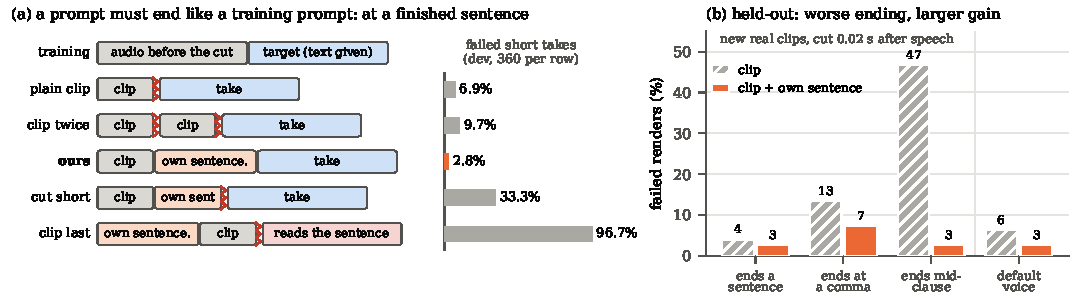
\includegraphics[width=\textwidth]{figures/fig_robust.pdf}
\caption{How the prompt ends decides whether a short sentence survives. (a) Prompt layouts (zig-zag: the
prompt stops mid-utterance) and the share of failed short takes on development units (30 sentences $\times$ 6
seeds $\times$ 2 voices = 360 per row, consensus judge). In training the text continues the prompt's utterance. Only a prompt ending at a finished sentence helps; more of the same clip does not, the same
extension cut short multiplies failures, and with the clip last the model reads the extension aloud.
(b) Held-out: new real clips cut 0.02\,s after their last sound, by where they end, and the engine's
default voice; the less finished the clip's ending, the larger the gain.}
\label{fig:robust}
\end{figure*}

\textbf{Prompt self-extension.} In training the text always continues the prompt's utterance; at inference
it never does. A reference clip cut right after its last phoneme, usually mid-utterance, therefore asks
for a continuation of \emph{its} utterance that the given words cannot provide, and short targets, with
the least room to recover, suffer most. Among training cuts, only those that happen to fall at a sentence
boundary have a new sentence as their continuation; a prompt that ends at a finished sentence puts every
inference into that case. We do not claim that training prompts typically end at sentences --- most
random word boundaries fall inside one --- but that this is the subset whose continuation matches ours. Once per voice, the model reads one neutral sentence
(\fa{«امروز هوا کمی سرد است و باد می‌وزد.»}, ``it is a little cold today and the wind blows'') from the
plain clip four times with fixed seeds; the take of median speech length (no recogniser) is kept, as raw
latents, up to its speech end plus one frame. Every later unit is conditioned on the clip followed by the
last $(5\,\text{s} - |\text{clip}|)$ of this extension. The prompt is encoded once into the key--value cache
that every unit already copies, so a request costs nothing extra.

\textbf{It is the ending that matters} (Fig.~\ref{fig:robust}a). On 30 short development sentences
$\times$ 6 seeds for each of two voices (male 1.36\,s and female 2.0\,s clip; 360 paired takes per layout),
the extension cuts failures from \RES{25} to \RES{10}. Repeating the clip, which adds speech
but keeps the abrupt ending, does not help (\RES{35}); the same extension cut after two thirds --- same voice,
same latents, unfinished --- multiplies failures (\RES{120}); and with the clip placed last the model reads the
extension aloud instead of the text in \RES{94--99\%} of takes (\fa{«بله»} comes out as
\fa{«امروز هوا کمی سرد ...»}). Teacher-forcing a carrier word, or priming each unit with the previous unit's
tail, adds nothing. Which sentence is read matters (two of seven candidates helped both voices) and was fixed
on development data.

\begin{table}[t]
\caption{Prompt self-extension, held-out (paired renders; change with 95\% CI)}\label{tab:robust}
\centering
\footnotesize
\setlength{\tabcolsep}{2.4pt}
\begin{tabular}{lccc}
\toprule
measure & clip & clip + ext. & change [CI] \\
\midrule
\multicolumn{4}{l}{\emph{short set: 50 fa + 10 Eng./mixed sentences $\times$ 6 seeds $\times$ 3 voices}} \\
failed renders (of 900 fa) & \RES{24} & \RES{12} & \\
consensus CER & \RES{.032} & \RES{.022} & \RES{$-$.011 [$-$.017, $-$.004]} \\
\quad default voice (1.36\,s clip) & \RES{.060} & \RES{.039} & \RES{$-$.021 [$-$.036, $-$.008]} \\
UTMOS / spk.\ change (1{,}080) & & & \RES{+.13 / $-$.012} \\
\quad speaker-matched extension take & & & \RES{+.18 / +.009} \\
\midrule
\multicolumn{4}{l}{\emph{3 new real clips cut 0.02\,s after speech; 50 fa sentences, 3 seeds}} \\
failed renders (of 450) & \RES{96} & \RES{19} & \RES{$-$.167 [$-$.233, $-$.106]} \\
\quad clip ending mid-clause, CER & \RES{.441} & \RES{.030} & \RES{$-$.411 [$-$.546, $-$.288]} \\
\midrule
\multicolumn{4}{l}{\emph{nine more speakers (ShEMO), 50 fa sentences $\times$ 2 seeds}} \\
failed renders (of 900) & \RES{69} & \RES{28} & \\
consensus CER & \RES{.070} & \RES{.033} & \RES{$-$.037 [$-$.053, $-$.024]} \\
UTMOS / spk.\ change & & & \RES{$-$.12 / $-$.021} \\
\midrule
\multicolumn{4}{l}{\emph{bench: 79 mixed cases $\times$ 3 seeds (55 fa cases scored)}} \\
consensus CER & \RES{.029} & \RES{.023} & \RES{$-$.006 [$-$.010, $-$.001]} \\
pitch reset at chunk joins (st) & \RES{5.25} & \RES{3.92} & \RES{$-$1.33 [$-$1.95, $-$.77]} \\
\midrule
\multicolumn{4}{l}{\emph{default voice, one take instead of the 3-take retry loop}} \\
consensus CER & \RES{.060} & \RES{.041} & \RES{$-$.019 [$-$.033, $-$.006]} \\
generations per unit & \RES{2.1} & \RES{1.0} & \\
\bottomrule
\end{tabular}
\end{table}

\textbf{Held-out results} (Table~\ref{tab:robust}, Fig.~\ref{fig:robust}b). On 60 unseen short sentences
rendered through the full production path, failed renders halve and UTMOS rises for every voice. The
prediction of the mechanism holds on three \emph{new} real clips cut 0.02\,s after their last sound: the
sentence-final clip improves slightly, the comma clip halves its error, and the mid-clause clip, nearly
unusable alone, becomes ordinary --- although the mid-clause clip ends at a word boundary just as training
prompts do, which is why we place the mechanism in what the text must continue, not in the cut itself. On a mixed bench of long and code-mixed text, error also falls, and units
of one sentence sound less like separate sentences (smaller pitch reset at joins). With the extension a single
take beats the engine's three-take loop, so retries can be dropped and the generation work halves; on 40
assistant-style replies this configuration is no worse on any measure with \RES{28\%} fewer generations.
The cost is speaker similarity on one voice (female, \RES{$-$0.03}); choosing the extension take by speaker
similarity removes it (\RES{+0.009} pooled) at part of the intelligibility gain. English sentences, read
through mapped Persian phonemes, keep the plain clip.

\textbf{Nine more speakers.} To test generality beyond our voices we took nine further speakers from ShEMO
(neutral clips of 2--5\,s, five male and four female, chosen so that no two WeSpeaker embeddings exceed a
cosine of \RES{0.38}), built their extensions automatically and rendered the short set twice per voice. Failed
renders fell from \RES{69} to \RES{28} of \RES{900} and the consensus error from \RES{7.0\%} to \RES{3.3\%}
(change \RES{$-$3.7} points, CI \RES{[$-$5.3, $-$2.4]}). The gain was significant for five voices, largest for
the two whose plain clips failed most (\RES{30$\to$3} and \RES{10$\to$1} failures); three were unchanged and one
got worse (\RES{1$\to$10} failures), so the extension is a strong default but not a guarantee for every clip.
On these radio-play voices it also costs naturalness and voice fidelity: UTMOS \RES{$-$0.12} pooled (up for
three voices, down for six) and speaker similarity \RES{$-$0.021}. Choosing the extension take by speaker
similarity, which removed this cost on our voices, was not applied here.

\textbf{A second model.} Qwen3-TTS-0.6B-Base \cite{qwen3tts2026} also clones a voice by continuation, from the
reference audio \emph{and} its transcript, over discrete 12\,Hz codec tokens. We built its extension the same
way (median of four readings of the same sentence, appended with its transcript) and rendered 25 held-out
short sentences $\times$ 2 voices. Persian is not a supported language of Qwen3-TTS and its error is about
ten times higher than our engine's; failed renders went from \RES{12} to \RES{10} of \RES{50} (error change
\RES{+1.4} points, CI \RES{[$-$7.1, +9.9]}, no measurable effect) while UTMOS rose by \RES{0.26} for both
voices (\RES{+0.16}, \RES{+0.36}) at unchanged speaker similarity (\RES{$-$0.006}). Both of those clips already
end at a finished sentence, so the mechanism predicts no intelligibility gain there --- as for our 5.1\,s
clip --- while the naturalness gain carries over to a different architecture.

\textbf{A first listening check.} A native Persian listener compared plain and extended prompts blind: \RES{60} pairs of
held-out short sentences in the default voice, same seed, left/right at random, choosing the better reading
or ``same'' and marking any word error. Preference did not differ (same \RES{33}, plain \RES{15}, extended
\RES{12}; sign test $p=\RES{.70}$); word errors were marked in \RES{7} plain and \RES{5} extended renders
(\RES{3} vs.\ \RES{1} on Persian-only sentences). None of the \RES{12} takes the listener marked was among the
\RES{9} the recognisers failed: errors on such short sentences are rare and idiosyncratic, so the recogniser-measured gain needs a larger listening test to be confirmed by ear.

\section{Expressiveness: What the Prompt Carries}\label{sec:expr}
\textbf{Diagnosis.} Because the model never sees a mark, a yes/no question and its statement twin are the
same audio sample for sample (final-pitch difference \RES{0.00}\,st; \RES{4.75}\,st in real speech). What the
words carry, the model does reproduce: on wh-questions it accents the question word (\RES{+3.4}\,st; real
\RES{+3.8}). Real speech also shows what else is missing (Fig.~\ref{fig:expr}e,\,f): renders of exclamations
lose \RES{5.7}\,dB of energy from their first to their second half, while ShEMO's neutral, surprised and happy
speech loses \RES{4.0}, \RES{1.8} and \RES{0.6}\,dB; real wh-questions end level (\RES{$-$0.9} to
\RES{$-$1.4}\,st) but ours fall like statements (\RES{$-$4.4}); and Persian alternative questions
(\fa{«چای یا قهوه؟»}) fall. A first remedy --- reshaping the whole contour of questions and exclamations by
TD-PSOLA --- gives questions a final rise but costs \RES{0.24} UTMOS on exclamations, an audible roughness,
and is barely heard: Whisper writes \fa{«؟»} for \RES{4\%} of such questions. Looking for a pitch direction
inside the model failed: a linear F0 probe on Mimi latents explains \RES{30\%} of the variance, but pushing
latents along it changed nothing until the sound broke.

\begin{figure*}[t]
\centering
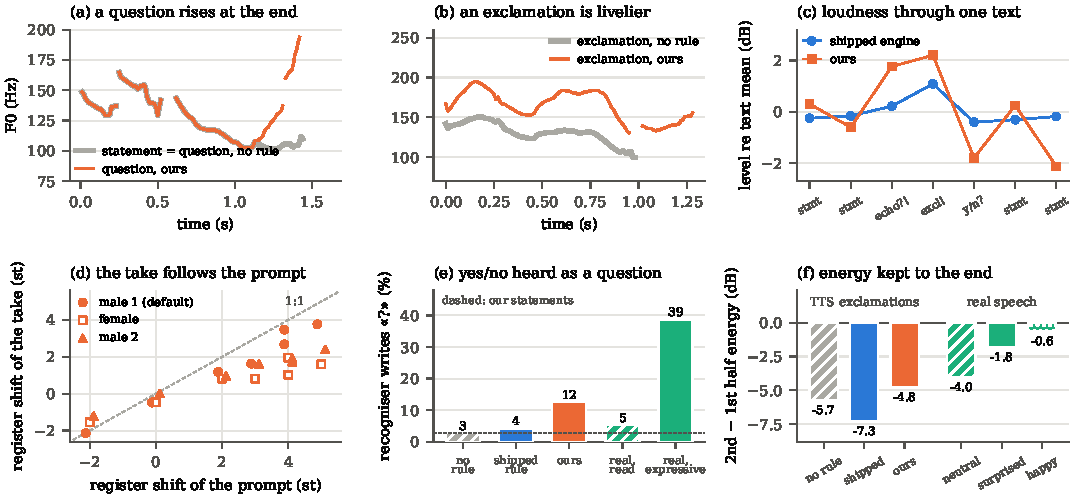
\includegraphics[width=\textwidth]{figures/fig_expr.pdf}
\caption{Expressiveness from the prompt, endings from the rule (held-out sentences unless noted).
(a) A yes/no question and its statement twin are one rendering for the model; the rule adds the final rise.
(b) An exclamation generated from the lively prompt: higher and wider throughout, with no processing of its
body. (c) Sentence loudness through one text, shipped engine vs.\ ours. (d) Register of the take against the
register shift of the styled prompt (development, three voices). (e) Yes/no questions heard as questions by
Whisper, vs.\ real read and expressive speech. (f) Energy of the second half of a sentence relative to the
first: our exclamations against real speech by emotion (ShEMO).}
\label{fig:expr}
\end{figure*}

\textbf{The prompt carries register and pitch range.} Since the model continues its prompt, we let the prompt
do the expressive part. The self-extension is decoded, its F0 raised by $r$\,st with excursions scaled by $k$
(TD-PSOLA), its level raised by $g$\,dB, and it is encoded back with the Mimi encoder; the take is generated
from the clip followed by this \emph{styled} extension and decoded as usual. On \RES{108} development renders
the take follows the prompt's register --- from a quarter to all of the shift, least for the female voice
(Fig.~\ref{fig:expr}d) --- and with $(r,k,g)=(4,1.6,4)$ its pitch range widens from \RES{9.0} to
\RES{12.2}\,st with consensus error, UTMOS, DNSMOS SIG and speaker similarity unchanged (\RES{$-$0.001},
\RES{+0.07}, \RES{+0.01}, \RES{$-$0.001}). A decode--encode round trip alone moves register by at most
\RES{0.5}\,st. Stronger styling begins to cost intelligibility, and for a voice whose extension lies above
165\,Hz the register shift is halved (on the female voice $r=4$ cost \RES{0.40} UTMOS on exclamations, $r=2$
\RES{0.12}). This \emph{lively} prompt is used for exclamations and surprised questions; a milder one for all
questions widened the range so much that it deepened the fall before the final rise (yes/no heard as
questions \RES{12\%$\to$7\%}) and was dropped. Each styled prompt is built once per voice (\RES{0.5}\,s).

\textbf{The rule restores only the ending.} From its written mark, interjections and question words the front
end types each sentence: statement, yes/no question (with tag questions), wh-question, alternative question,
surprised or echo question (\fa{«جدی؟»}, \fa{«؟!»}), and exclamation with an intensity that grows with
\fa{«!!»} and interjections. A yes/no question rises over its \emph{last syllable} only --- found as the energy
valley before the last vowel nucleus --- along $u^{1.3}$ to 9\,st above the median, and that syllable is
lengthened by 15\%; a surprised question rises to 8\,st; the final fall of wh-questions and exclamations is
stopped at $-1$\,st; alternative questions are left to fall; and the second half of questions and
exclamations is raised by up to 2 and 3.5\,dB with a plain gain envelope, as in excited speech. Over a text,
exclamations gain +3\,dB times their intensity, surprised questions +2, other questions +0.5, and a
paragraph's first and last sentences +1 and $-$1.5\,dB; a look-ahead peak limiter keeps the plan intact where
scaling a whole sentence down would undo it. These settings were chosen on development sentences by the
recogniser-heard question rate against UTMOS.

\begin{table}[t]
\caption{Expressiveness, held-out (3 voices $\times$ 2 seeds; 348 question and exclamation renders) and whole
texts (8 texts, 48 renders). Shipped: contour rule alone; ours: lively prompt + ending rule + plan}\label{tab:expr}
\centering
\footnotesize
\setlength{\tabcolsep}{2.0pt}
\begin{tabular}{lccc}
\toprule
measure & no rule & shipped & ours \\
\midrule
yes/no heard as question (\fa{«؟»}) & \RES{3\%} & \RES{4\%} & \RES{12\%} \\
yes/no $-$ statement, final F0 (st) & \RES{0.00} & \RES{+3.63} & \RES{+3.56} \\
alt.\ questions, final F0 (st) & \RES{$-$0.40} & \RES{+2.68} & \RES{$-$0.40} \\
wh-questions, final F0 (st) & \RES{$-$4.35} & \RES{$-$4.35} & \RES{$-$2.99} \\
surprised q., register (st) & 0 & \RES{+1.05} & \RES{+3.65} \\
exclam., pitch range (st) & \RES{7.5} & \RES{7.1} & \RES{10.4} \\
exclam., level (dB) & 0 & \RES{+0.7} & \RES{+2.2} \\
exclam., 2nd$-$1st half energy (dB) & \RES{$-$5.7} & \RES{$-$7.3} & \RES{$-$4.8} \\
texts: sentence level SD (dB) & \RES{0.49} & \RES{0.67} & \RES{1.31} \\
texts: sentence register SD (st) & \RES{1.22} & \RES{1.20} & \RES{1.61} \\
\midrule
consensus CER (fails) & \RES{.041 (9)} & \RES{.043 (10)} & \RES{.041 (8)} \\
$\Delta$UTMOS, all / exclam. & & \RES{$-$.12 / $-$.24} & \RES{$-$.10 / $-$.02} \\
$\Delta$SIG / $\Delta$speaker sim. & & \RES{$-$.028 / $-$.002} & \RES{$-$.040 / $-$.009} \\
texts, ours$-$shipped: CER/UTMOS & & & \RES{$-$.001 / $-$.03} \\
\bottomrule
\end{tabular}
\end{table}

\textbf{Results} (Table~\ref{tab:expr}, Fig.~\ref{fig:expr}). Yes/no questions are heard as questions three
times as often as with the contour rule (\RES{12\%} vs.\ \RES{4\%}; read speech \RES{5\%}, expressive
\RES{39\%}) at the same rise over their statement twins; alternative questions keep their fall;
wh-questions end \RES{1.4}\,st higher, toward real speech; surprised questions are spoken \RES{3.7}\,st higher
and \RES{1.9}\,dB louder; exclamations come out with a \RES{38\%} wider pitch range, \RES{2.2}\,dB louder,
with their energy kept up between real neutral and excited speech, at almost no UTMOS cost (\RES{$-$0.02}
against \RES{$-$0.24}). Through whole texts, sentence loudness varies twice as much as before
(\RES{0.67$\to$1.31}\,dB; read speech \RES{1.52}) and register a third more. Intelligibility is unchanged. The
costs are a small loss of speaker similarity on exclamations (\RES{$-$0.028}) and of UTMOS on surprised one-
and two-word questions (\RES{$-$0.25}), where both the rise and the prompt act on very little audio.

\textbf{Nine more speakers.} On the nine ShEMO voices of Sec.~\ref{sec:robust} (held-out sentences, one seed,
522 renders per system) the comparison with the shipped engine holds in direction and the quality cost
disappears: UTMOS rises overall (\RES{+0.08}, CI \RES{[+0.04, +0.11]}) and most on exclamations (\RES{+0.30}),
which also come out \RES{3.3}\,dB louder with their energy kept up (\RES{$-$6.6$\to$$-$4.2}\,dB); surprised
questions are spoken \RES{2.8}\,st higher and end \RES{2.4}\,st higher; wh-questions end \RES{0.9}\,st higher;
alternative questions fall again (\RES{+1.7$\to$$-$1.0}\,st) and are heard as yes/no questions less often
(\RES{36\%$\to$22\%}); the question--statement gap stays (\RES{+2.8}\,st). Two effects are weaker on these
voices: the register lift of exclamations (\RES{+0.3}\,st) and the recogniser's question rate for yes/no
questions (\RES{5\%$\to$6\%}, n.s.).

\textbf{What did not improve clarity.} The default voice renders \RES{10}\,dB weaker at 2.5--6\,kHz than its
own clip, but equalising each render toward the clip lowered UTMOS and DNSMOS SIG (\RES{$-$0.06} each);
equalising the prompt instead brightened the take by \RES{4.5}\,dB at a cost in speaker similarity; pitch marks
from zero-frequency filtering \cite{zff2008} made TD-PSOLA rougher on codec speech (UTMOS \RES{$-$0.37} vs.\
\RES{$-$0.27} for a flat +2\,st shift); and re-encoding processed audio with the codec hid the processing cost
but cost \RES{2.1} points of error. The clarity gain that held up was structural: moving the expressive
work from the signal into the prompt.

\textbf{Listening.} Besides the blind check of Sec.~\ref{sec:robust}, the authors listened to every held-out
question and exclamation and to the eight texts in both versions, shipped and ours, and preferred ours
throughout: yes/no questions are heard as questions, surprise and exclamations as such, alternative questions
fall, and loudness moves through a text instead of staying flat; the labelled pages are released with the
code. A formal blind test for 20--30 native listeners is designed and released with it as well: sentence-type
identification with the final mark hidden, naturalness MOS and CMOS, clarity of short replies, and
inter-rater agreement (Krippendorff's $\alpha$, Fleiss' $\kappa$), with a script that scores it.

\section{Discussion and Limitations}\label{sec:discussion}
\textbf{One mechanism, two uses.} Both methods follow from how the model was trained: the prompt was the
start of the very utterance the target completes. Ending the prompt at a finished sentence makes ``a new
sentence'' a valid continuation, as at the sentence-boundary cuts of training; a prompt that stops
mid-phrase asks the model to finish something it was not given the words for, and short targets come out
truncated or replaced by a replay of the prompt. How often training cuts fell at sentence boundaries we could
not measure, because the training manifests are not public. And because the model learned to continue a speaker, it
continues that speaker's register and liveliness too --- so the prompt can carry delivery the text cannot. The
same reasoning applies to any continuation TTS model (the naturalness gain held on Qwen3-TTS), and the split of labour --- prompt for the body of a
sentence, a rule for its boundary tone --- to any model trained on text without punctuation.

\textbf{Limitations.} One model is tuned and evaluated in depth, on thirteen speakers; a second model was
tested only for robustness, on 50 renders. Perceptual evidence so far is one
blind listener for robustness and the authors' own listening for expressiveness; the released multi-listener
test is the next step. Expressiveness is also measured acoustically and
through one recogniser whose question rate is itself only \RES{39\%} on real expressive speech; the
expressive reference (ShEMO) is acted radio speech whose texts we attached by recogniser matching
(\RES{279} of \RES{760} clips) and which has no speaker labels. Style strengths and the extension sentence are
hyperparameters chosen on few development renders.

\section{Conclusion}\label{sec:conclusion}
A small CPU TTS model can be made both more robust and more expressive without training, through the one
input that carries acoustics into the model: its voice prompt. Ending the prompt at the model's own finished
sentence halves failed short renders, rescues clips cut mid-utterance and lets the engine drop its retries.
Re-styling that sentence makes the model itself speak exclamations and surprise higher and livelier, so the
signal processing shrinks to sentence endings and a loudness plan, and questions are heard as questions three
times as often at no loss of intelligibility. A two-recogniser consensus and a recogniser used as a listener
made both effects measurable. The engine, sets and scripts are available at \CODEURL.

\bibliographystyle{IEEEtran}
\bibliography{refs}
\end{document}
